\documentclass[tikz,border=2pt]{standalone}
\usepackage{amsmath,amssymb}
\usepackage{tikz}
\usetikzlibrary{arrows.meta}

\begin{document}
% 1/z = conj(z)/|z|^2: reflect z in the real axis and invert its modulus, so points outside
% the unit circle land inside it and vice versa.
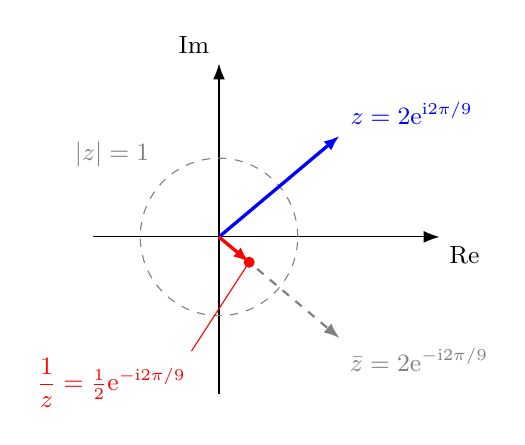
\begin{tikzpicture}[every node/.style={font=\small}, >={Latex[length=2mm]}]
	\draw[->] (-1.6,0) -- (2.8,0) node[below right] {$\mathrm{Re}$};
	\draw[->] (0,-2.0) -- (0,2.2) node[above left] {$\mathrm{Im}$};
	\draw[gray, dashed] (0,0) circle (1);
	\node[gray, anchor=south east, font=\small] at (135:1.08) {$|z|=1$};
	\draw[->, blue, very thick] (0,0) -- (40:2) node[above right] {$z=2\mathrm{e}^{\mathrm{i}2\pi/9}$};
	\draw[->, gray, thick, dashed] (0,0) -- (-40:2) node[below right] {$\bar z=2\mathrm{e}^{-\mathrm{i}2\pi/9}$};
	\draw[->, red, very thick] (0,0) -- (-40:0.5);
	\fill[red] (-40:0.5) circle (2pt);
	\draw[red, thin] (-40:0.5) -- (-0.35,-1.45);
	\node[red, anchor=north east] at (-0.3,-1.42) {$\dfrac1z=\tfrac12\mathrm{e}^{-\mathrm{i}2\pi/9}$};
\end{tikzpicture}
\end{document}
